\chapter{Lecture}\label{part3:lec27}%%% 27
\markboth{\thechapter. Lecture}{\thechapter. Lecture}

We\pageoriginale now give a proof of the transformation formula for
$\eta(\tau)$. $\eta(\tau)$ we first introduced by Dedekind in his
commentary on a fragment on modular functions by Riemann; it is
natural in the theory of elliptic functions.
$$
\eta (\tau) = e^{\frac{\pi i \tau}{12}} \prod^\infty_{m=1} (1- e^{2
  \pi i m \tau})
$$ 

We want to replace $\tau$ by $\tau' = \dfrac{a \tau+b}{c \tau
  +d}$. Actually in the whole literature there is no full account
except in a paper by W.Fischer (Pacific Journal of Mathematics,
Vol. 1). We know what happens in the special cases $- \frac{1}{\tau}$
and $\tau+1$. We get the explicit form in which the root of unity
appears in the transformation formula if we put together some things
from the theory of modular functions. There some discussion in
Tannery-Molk; they write $h(\tau)$ instead of
$\eta(\tau)$. $(\eta(\tau))^3$ is up to a factor $\mathscr{V}_1^1 (o
/\tau)$. It turns out for quite other reasons that $(\eta (\tau))^8$
can be discussed too; it has to do with the modular invariant
$J(\tau)$. Dedekind did something more than what is needed
here. He studied $\log \eta(\tau)$. For $\im \tau > 0$, $\eta(\tau)$
is a function in the interior of the unit circle (if we set $x= e^{2
  \pi i \tau}$) free from zeros and poles. So the logarithm has no
branch points and is fully defined without ambiguity.
$$
\log \eta(\tau) = \frac{\pi i \tau}{12} + \sum^\infty_{m-1} \log (1-
e^{2 \pi i m \tau})
$$ 

(For purely imaginary $\tau$, the logarithms on the right side are
real). 

The\pageoriginale multiplicative root of unity now appear as
something additive. This is what Ded\'ekind investigated. Recently
(Mathematika, vol.1, 1954) Siegel published a proof for the particular
case $-\dfrac{1}{\tau}$, using logarithms. Actually Siegel proves much
more than the functional equation for $\eta(\tau)$. He proves that
$$
\log \eta (- \tau^{-1})= \log \eta (\tau)+ \frac{1}{2} \log \frac{\tau}{i}
$$ 

We shall extend his proof to the more general case. The interesting
case where a root of unity appears explicitly has not been dealt with
by Siegel.

We write the general modular transformation in the form
$$
\tau = \frac{h+ i \mathfrak{z}}{k}, \tau' = \frac{h' + i
  /\mathfrak{z}}{k}, h h' \equiv -1 \pmod{k}
$$

We wish to prove that
\begin{equation*}
  \log \eta \left( \frac{h' + i/\mathfrak{z}}{k}\right) = \log \eta
  \left(\frac{h+ i \mathfrak{z}}{k} \right) + \frac{1}{2} \log
  \mathfrak{z} + \pi i C(h, k)\tag{*}\label{part3:lec27:eq*}
\end{equation*}
where $C(h, k)$ is a real constant.

From the definition of $\eta (\tau)$, 
\begin{align*}
  \log \eta \left( \frac{h+ i \mathfrak{z}}{k}\right) & = \frac{\pi
    (h+ i \mathfrak{z})}{12k} - \sum^\infty_{m=1} \sum^\infty_{r=1}
  \frac{1}{r} e^{2 \pi i m r (h + i \mathfrak{z})/k}\\
  & = \frac{\pi i h}{12k} - \frac{\pi \mathfrak{z}}{12k} -
    \sum^\infty_{m=1} \sum^\infty_{r=1} \frac{1}{r} e^{2 \pi i m r
      h/k} e^{- 2 \pi m r \mathfrak{z}/k}
\end{align*}
$e^{2 \pi i m r h/k}$\pageoriginale is periodic with period $k$; we emphasize this
and write
$$
m= qk+ \mu; \mu=1, \ldots, k; q=0, 1, 2, \ldots.
$$

Then
$$
\log \eta \left( \frac{h+ i \mathfrak{z}}{k}\right) = \frac{\pi i
  h}{12 k} - \frac{\pi \mathfrak{z}}{12k} - \sum^\infty_{q=0}
\sum^k_{\nu=1} \sum^\infty_{r=1} \frac{1}{r} e^{2 \pi i \mu \frac{r
    h}{k}} e^{- 2 \pi (1 k+ \mu) \frac{r \mathfrak{z}}{k}},
$$
and taking the summation over $q$ inside, this becomes
\begin{multline*}
  \frac{\pi i h}{12k} - \frac{\pi \mathfrak{z}}{12k} -
  \sum^\infty_{\mu=1} \sum^\infty_{r=1} \frac{1}{r} e^{2 \pi i \mu
    \frac{r h}{k}} e^{- 2 \pi \mu \frac{r\mathfrak{z}}{k}}
  \sum^\infty_{q=0} e^{- 2 \pi q r \mathfrak{z}}\\
  = \frac{\pi i h}{12k} - \frac{\pi \mathfrak{z}}{12k} -
  \sum^k_{\mu=1} \sum^\infty_{r=1} \frac{1}{r} e^{2 \pi i \mu \frac{r
      h}{k}} \frac{e^{- 2 \pi \mu r\mathfrak{z}/k}}{1- e^{-2 \pi r \mathfrak{z}}}
\end{multline*}

Substituting in (\ref{part3:lec27:eq*}), with similar expansion for
$\eta \left(\frac{h' + i/\mathfrak{z}}{k}\right)$, we have
\begin{multline*}
  \frac{\pi i h}{12k} - \frac{\pi}{12k \mathfrak{z}} -
  \sum^k_{\nu=1} \sum^\infty_{r=1} \frac{1}{r} e^{2 \pi i \nu r
    \frac{h'}{k}} \frac{e^{-\frac{2 \pi \nu r}{k\mathfrak{z}}}}
  {1-e^{- 2 \pi  r/ \mathfrak{z}}}\\
  = \frac{1}{2} \log \mathfrak{z} + \pi i C(h, k) + \frac{\pi i
    h}{12k} - \frac{\pi 
  \mathfrak{z}}{12k} -\sum^k_{\mu=1} \sum^\infty_{r=1} \frac{1}{r}
  e^{2 \pi i \mu \frac{r h}{k}} \frac{e^{- 2 \pi \mu
      \frac{r\mathfrak{z}}{k}}}{1- e^{-2 \pi r \mathfrak{z}}}  
\end{multline*}

Rearranging\pageoriginale this, we get
\begin{multline*}
  \sum^k_{\nu =1} \sum^\infty_{r=1} \frac{1}{r} e^{2 \pi i \nu r
    \frac{h'}{k}}. \frac{e^{- 2 \pi \nu r/k\mathfrak{z}}}{1- e^{-2 \pi
    r/\mathfrak{z}}} - \sum^k_{\mu =1} \sum^\infty_{r=1} \frac{1}{r}
  e^{2 \pi i\mu r h/k} \frac{e^{- 2 \pi \mu r \mathfrak{z}/k}}{1- e^{-
      2 \pi r/\mathfrak{z}}}\\
  + \frac{\pi}{12 k} \left( \frac{1}{\mathfrak{z}} -
  \mathfrak{z}\right) + \frac{\pi i}{12k} (h- h') + \pi i C(h, k) = -
  \frac{1}{2}  \log \mathfrak{z}.
\end{multline*}

We now follow Siegel's idea to get the whole thing as a sum of
residues of a certain function. Clearly there is $r$ in it. Being
integers $r$ can be produced by something like $\dfrac{1}{1- e^{2 \pi
  i x}}$ which has poles with residue $- \frac{1}{2 \pi i}$ at every
integral valued $x$. So let us study a function like
$$
\frac{1}{x} \frac{1}{1- e^{2 \pi i x}} e^{2 \pi i \mu x h/k} \frac{e^{-
  2 \pi \mu x \mathfrak{z}/k}}{1-e^{-2 \pi x \mathfrak{z}}}
$$

We may have to sum this from $\mu =1$ to $\mu =k$. This should somehow
be the form of the function that we wish to integrate. We do not want
it in the whole plane. In fact, we can either take a wider and wider
path of integration, or multiply the function by a factor
and\pageoriginale magnify it; we prefer to do the latter. We shall
put $xN$ for $x$, keep the path fixed and take $N= n + \frac{1}{2}$,
$n$ integer, to avoid integral points, and then make $n \to
\infty$. The term corresponding to $\mu =k$ should be treated
separately, as otherwise the factor $e^{- 2 \pi x \mathfrak{z}}$ would
stop convergence. Also $\mu^h$ and $\mu$ should appear symmetrically
for reasons which we shall see. So introduce $\mu^* \equiv \mu^h
\pmod{k}$, $\mu = 1, 2, \ldots, k-1$, and choose $1 \leq \mu^* \leq
k-1$. It turns out, taking all this together, that the following thing
will do. Write
$$
F_n (x) =- \frac{1}{4 ix} \cot h \pi N x \cot \frac{\pi N
  x}{\mathfrak{z}} + \sum^{k-1}_{\mu =1} \frac{1}{x} \cdot \frac{e^{2 \pi
    \mu Nx/k}}{1- e^{2 \pi N x}} \cdot  \frac{e^{- 2 \pi i \mu N x/k
    \mathfrak{z}}}{1-e^{-2\pi i N x/\mathfrak{z}}}
$$

The first term is a consequence of the term for $\mu = k$:
$$
\frac{1}{x} \times \frac{e^{2 \pi N x i}}{1- e^{2 \pi i x N}} \times
\frac{e^{- 2 \pi x N \mathfrak{z}}}{1- e^{- 2 \pi x N \mathfrak{z}}}
$$

The poles will not change if we write this as
\begin{align*}
  \frac{1}{x} \left(\frac{e^{2 \pi N x i}}{1- e^{2 \pi i N x}} +
  \frac{1}{2} \right) \left( \frac{e^{- 2 \pi x N \mathfrak{z}}}{1-
    e^{- 2 \pi x N \mathfrak{z}}} + \frac{1}{2}\right) & = \frac{1}{x}
  \frac{1 + e^{2 \pi i N x}}{2 (1- e^{2 \pi i N x})} \cdot \frac{1+
    e^{-2 \pi x N \mathfrak{z}}}{2(1-e^{- 2 \pi x N \mathfrak{z}})}\\
  & = \frac{1}{4 xi} \cot \pi  x N \cdot \cot h \pi x N \mathfrak{z}.
\end{align*}

We\pageoriginale integrate $F_n (x)$ along a certain parallelogram
$P$, a little different from Siegel's. $P$ has vertices at $\pm z$,
$\pm i$ (since $\mathcal{J}_m \tau > 0$, $\mathcal{R}_e \mathfrak{z} >
0$). Then
$$
\frac{1}{2 \pi i} \int_p F_n (x) dx = \sum (\text{Residues}).
$$
\begin{figure}[H]
  \centering{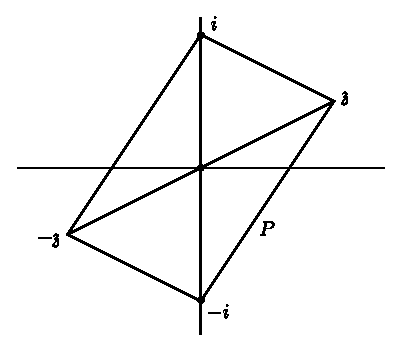
\includegraphics{vol2-figures/fig2.33.eps}}
\end{figure}

We then let $n \to \infty$.

The poles of $F_n (x)$ are indicated by the denominators and the
cotangent factors. These are 
$$
x= 0, \quad x=- \frac{r\mathfrak{z}}{N}, \quad x= \frac{i r}{N}, \quad
r \quad \text{integer}.
$$
$x=0$ is a triple pole for the first summand.
\begin{multline*}
- \frac{1}{4 i x} \cot h \pi N x \cot \frac{\pi N x}{\mathfrak{z}} =
- \frac{1}{4 ix} \cdot \frac{1}{\pi N x} \frac{\mathfrak{z}}{\pi N x}\\
\left\{ 1+ \frac{(\pi N x)^2}{3} + \cdot \right\}\times \left\{ 1-
\frac{(\pi N x/\mathfrak{z})^2}{3}+ \cdots \right\}
\end{multline*}

Residue\pageoriginale for this term at $x=0$
\begin{align*}
  & = \frac{i \mathfrak{z}}{4 \pi^2 N^2} \cdot \frac{1}{3} \left(
  \pi^2 N^2 - \frac{\pi^2 N^2}{\mathfrak{z}} \right)\\
  & = \frac{i}{12} \left( \mathfrak{z} - \frac{1}{\mathfrak{z}}\right).
\end{align*}
which had been foreshadowed already.
